\chapter{Introduction}

\section{Background}

Most of today's popular relational databases use a \emph{Volcano}-style iterator model \cite{Graefe:1994:VEP:627290.627558} for query processing. In this processing model, each operator (say, a projection, selection, join, etc.) produces a stream of tuples. The output stream of another operator is consumed using a simple interface, consisting only of the functions \texttt{open()}, \texttt{next()} and \texttt{close()}. Figure \ref{fig:volcano-processing} demonstrates this approach.

Whilst these databases benefit from a clean and flexible design which maximises maintainability and developer productivity, the Volcano-style processing model makes excessive use of function calls. For example, consider alone the \texttt{next()} call, which must be made for every tuple in the input, each intermediate result, and the final result. As main memory has grown, it is now often the CPU which determines query processing performance, and these function calls lead to frequent instruction mispredictions, and by extension control hazards, requiring CPU stalls which significantly degrade performance.

Database systems such as \emph{MonetDB} \cite{Boncz:2008:BMW:1409360.1409380} pioneered a bulk-processing approach, shown in figure \ref{fig:bulk-processing}, which, instead of considering one tuple at a time, considers entire columns at a time. The benefit of this approach is that the cost of calling the next operator is amortised over the number of tuples. However, it also introduces a new cost: intermediate results must now be materialised. Whilst the iterator-model can pipeline most operators (that is, the output of one operator can be passed directly to the input of the next), this is no longer possible with the bulk-processing model, which must make all resulting tuples accessible to the next operator to process at once. This often results in memory bandwidth constraining performance.

In an attempt to solve this, a new query engine, \emph{X100} \cite{DBLP:conf/cidr/BonczZN05} (which later evolved into VectorWise), was built for MonetDB, which processes smaller (say 1000-value) vectors, which form chunks of columns. These vectors can fit in the CPU cache, and can be pipelined to avoid expensive materialisation.

More recently, the \emph{HyPer} in-memory database system \cite{Neumann:2011:ECE:2002938.2002940} was shown to significantly outperform MonetDB and VectorWise in most cases, by using LLVM to compile queries into machine code with better locality and a more predictable branch layout. In this approach, chains of operators which can be pipelined (i.e. chains that do not require materialisation) are identified, and each of these fragments is compiled separately into machine code, as shown in figure \ref{fig:code-generation}. This reverses the direction of data-flow control: instead of each operator asking its input for tuples, each fragment of code processes the data and makes it available to the next fragment. Operators within each fragment leave tuples inside the CPU registers and so are extremely cheap, whilst pipeline-breaking operators (at the edge of fragments) would have required materialisation anyway, so there is no significant performance implication for them.

\begin{figure}
\centering
\begin{subfigure}[b]{0.49\textwidth}
    \centering
    \begin{tabular}{|c|}
    \hline
    \begin{lstlisting}[language=SQL]
SELECT
  "c_nationkey",
  COUNT("c_custkey")
    AS "customers_in_debt"
FROM
  "customer"
  JOIN "nation"
    ON "c_nationkey" = "n_nationkey"
WHERE
  "c_acctbal" < 0 
GROUP BY
  "c_nationkey"
    \end{lstlisting} \\
    \hline
    \end{tabular}
    \caption{A simple SQL query}
    \label{fig:simple-query}
\end{subfigure}
\begin{subfigure}[b]{0.49\textwidth}
    \centering
    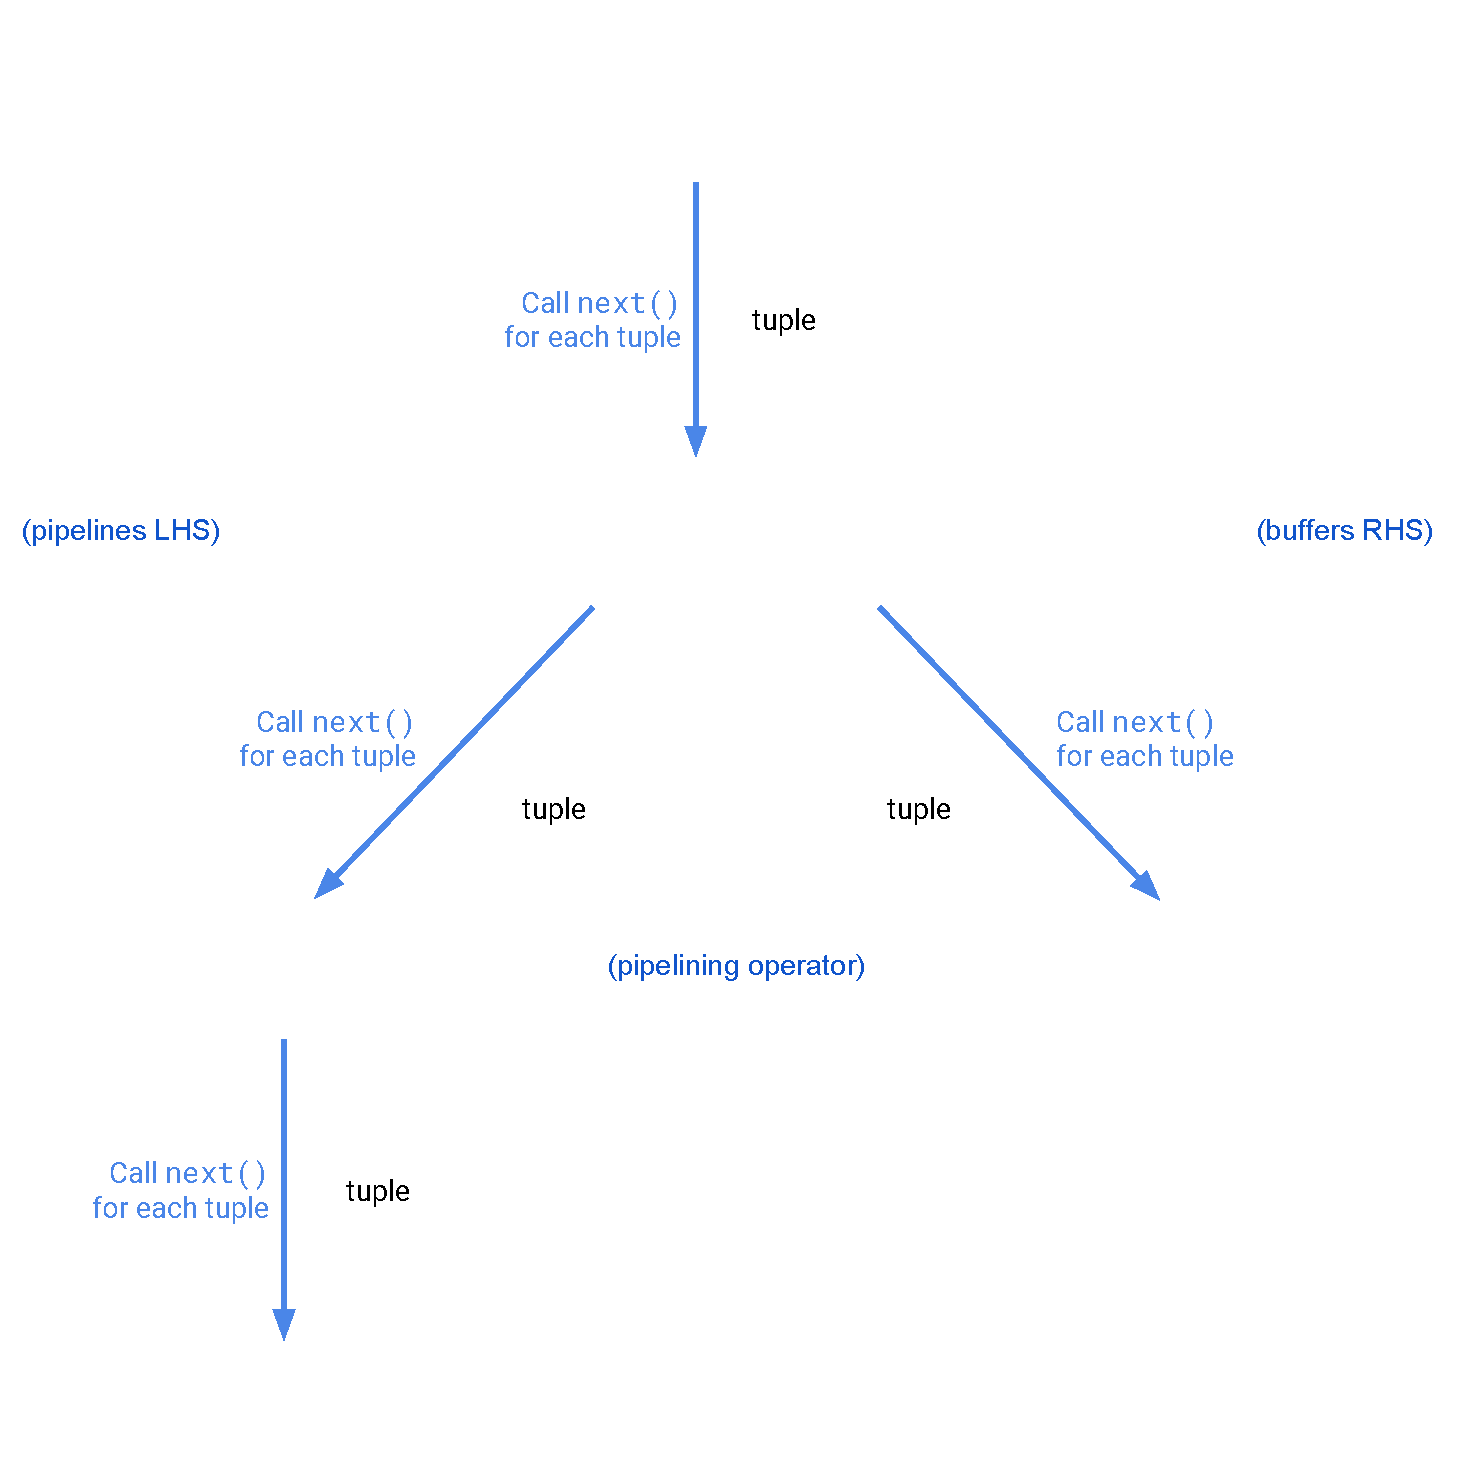
\includegraphics[width=0.9\linewidth]{introduction/volcano.pdf}
    \caption{Evaluating \ref{fig:simple-query} using Volcano processing}
    \label{fig:volcano-processing}
\end{subfigure}
\\[5ex]
\begin{subfigure}[b]{0.49\textwidth}
    \centering
    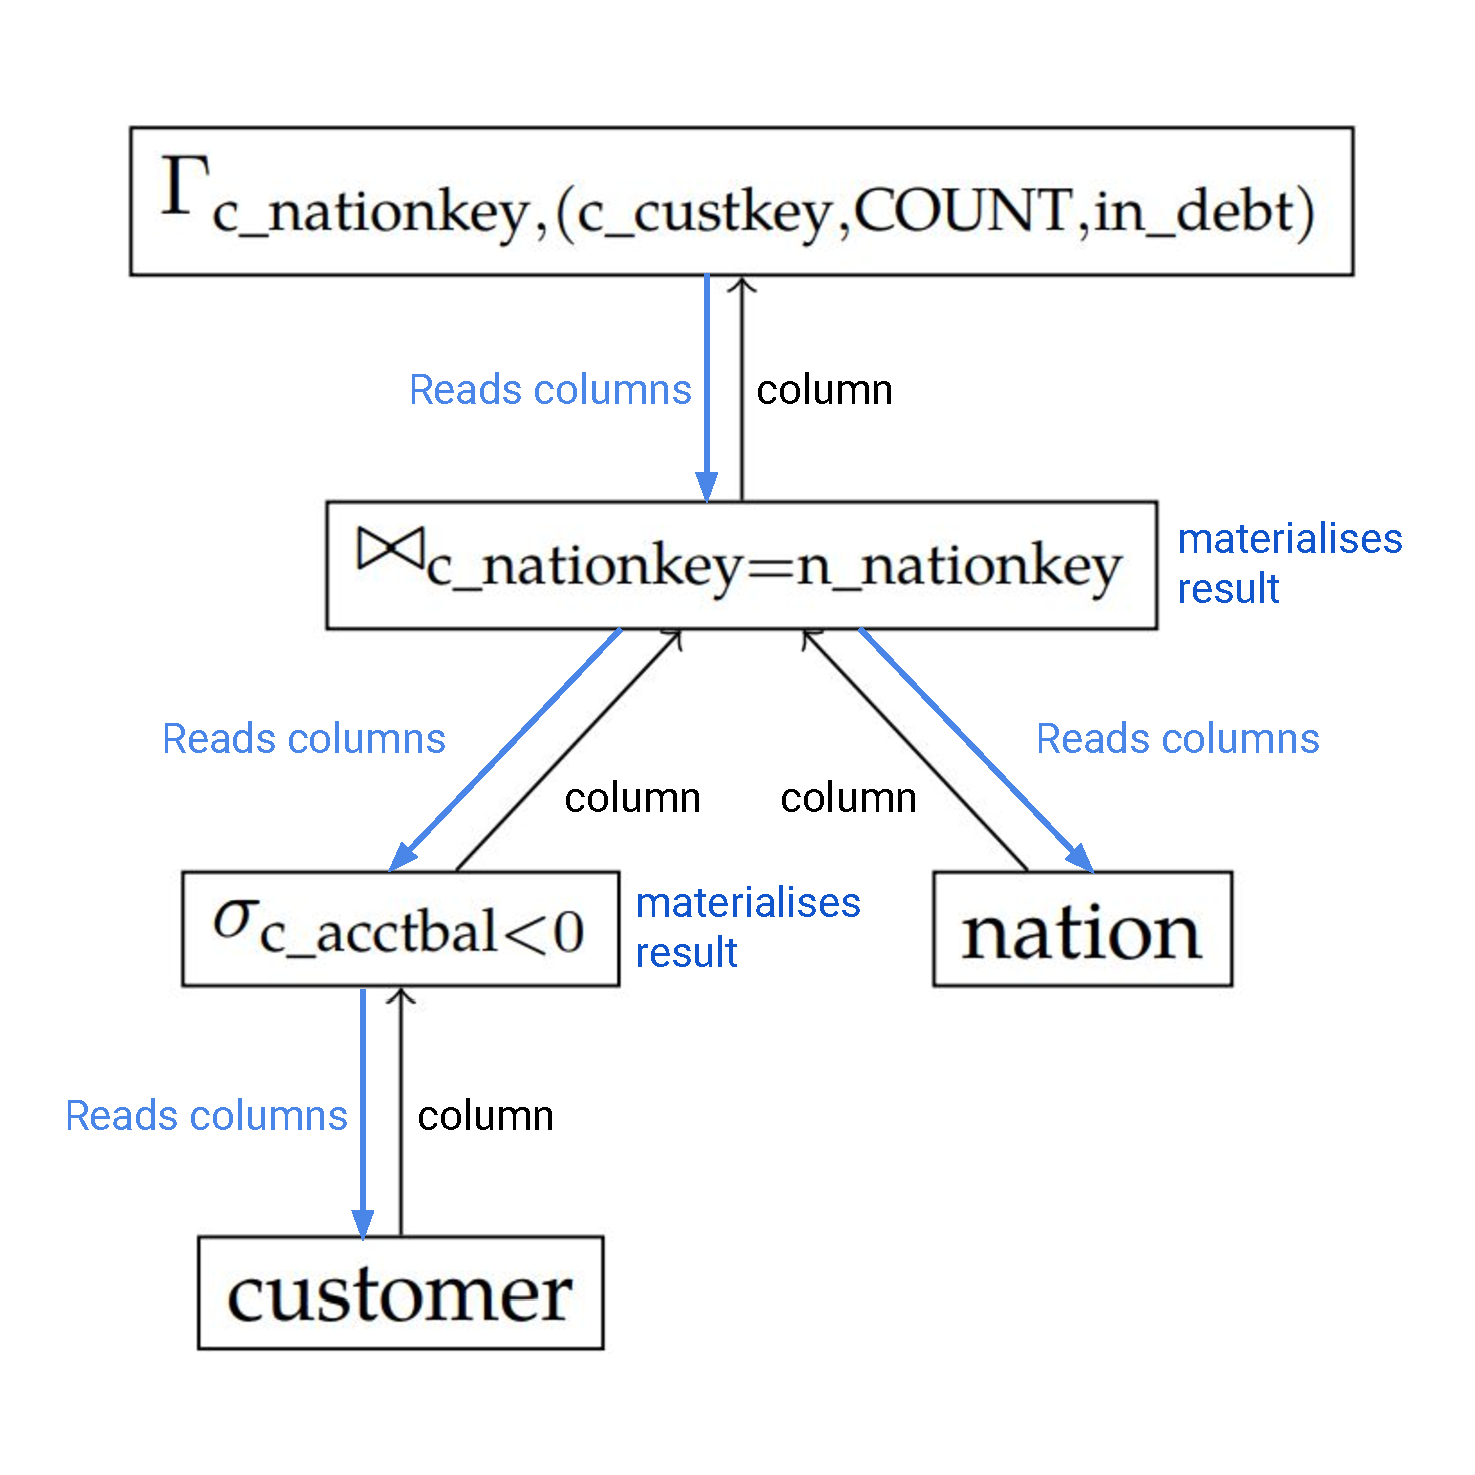
\includegraphics[width=0.9\linewidth]{introduction/bulk.pdf}
    \caption{Evaluating \ref{fig:simple-query} using bulk processing}
    \label{fig:bulk-processing}
\end{subfigure}
\begin{subfigure}[b]{0.49\textwidth}
    \centering
    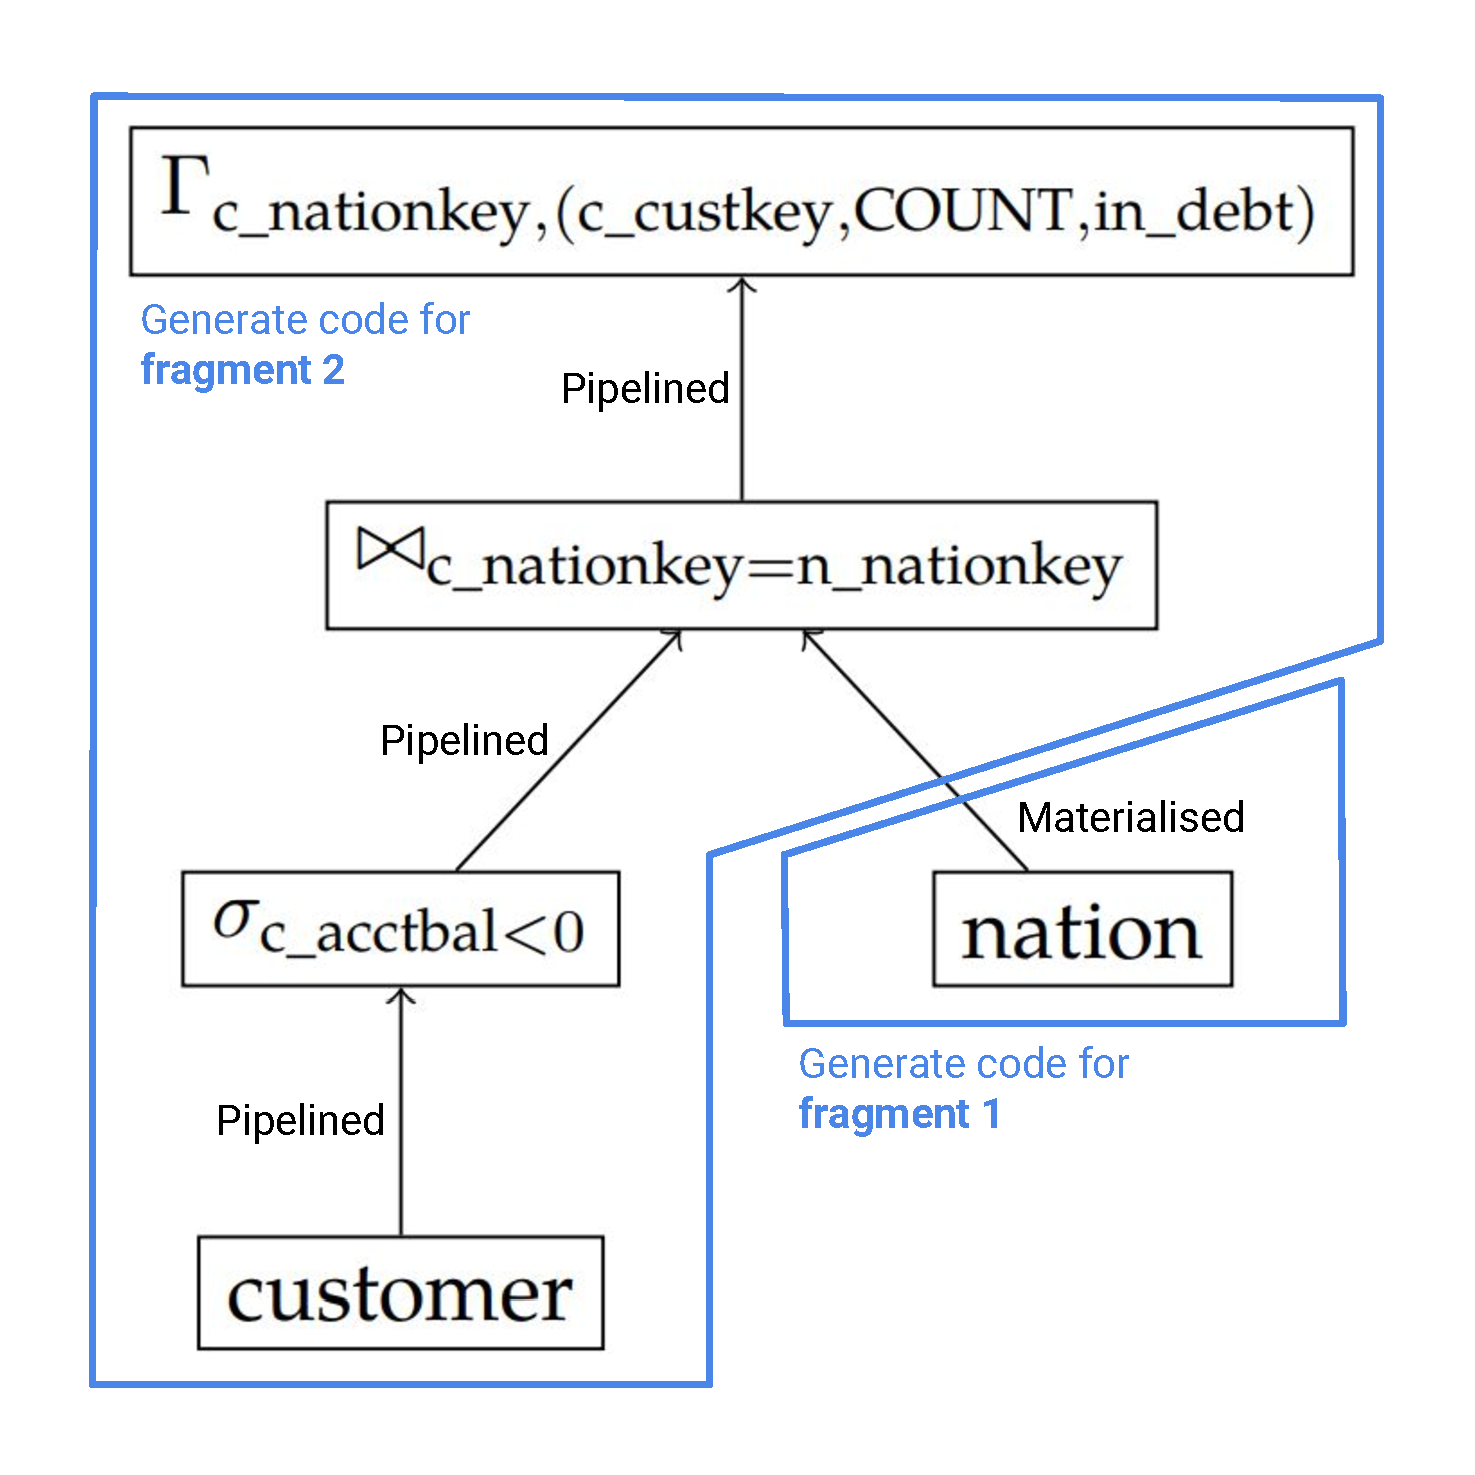
\includegraphics[width=0.9\linewidth]{introduction/codegen.pdf}
    \caption{Evaluating \ref{fig:simple-query} using code generation (the right input of the join would require its own fragment, if any operations were applied to the \texttt{nation} table)}
    \label{fig:code-generation}
\end{subfigure}
\caption{Approaches for improving query processing time}
\label{fig:improving-qpt}
\end{figure}

\emph{Voodoo} \cite{Pirk:2016:VVA:3007328.3007336} is a vector algebra which can be used as an intermediate representation between a database query and a code implementation, similar to what HyPer might produce. Voodoo allows the often data and hardware dependant kind of optimisations used in systems such as HyPer to be expressed in a portable way, and is designed to be \emph{tunable}, that is, it is able to express very simply most optimisations for in-memory query processing. It has been shown to generate highly-efficient OpenCL code to run on GPUs, outperforming existing state-of-the-art in-memory query processors for many queries.

\section{Motivation}

%Voodoo [https://pdfs.semanticscholar.org/45a9/1b4d9bcb2178c05e95685aca2f2aac94cdb0.pdf], is a high performance database kernel built around the idea of tunable, just-in-time compiled query execution. It is, arguably, the fastest database kernel right now. However, it is not a full data management system. It lacks an interactive query interface, a proper catalog manager, a logical query optimizer and many more components. In addition to that, it is built upon a fragile code generation process based on string concatenation. 

Whilst benchmarks have shown that using Voodoo allows some of the fastest query processing times out of any modern approach, it was not really available in a form that made it easy to use:

\begin{enumerate}
    \item The existing Voodoo implementation (detailed in \ref{original-voodoo-impl}) was a database \emph{kernel} meaning that it is far from being a full database management system.
    
    It was implemented as a replacement back-end for MonetDB. However the components to convert a query to a MonetDB plan remained separate to the Voodoo kernel itself, so there was no way to run queries, apart from TPC-H benchmarking queries, whose MonetDB plans were hard-coded into the driver program.
    
    \item The code generation itself was done by concatenating strings which formed the OpenCL program. This approach resulted in complex and fragile code, which was very difficult to extend. Importantly, once code had been written to the string, it could not be altered anymore so the program could only be written from top to bottom. This led to some optimisation strategies for the generated code being difficult or impossible to implement. 
    \item Certain parts of the code also suffered from particularly sparse documentation, and several bugs which were identified during this project.
\end{enumerate}

\section{Objectives}

This project essentially has two main goals: to replace the existing code generation engine with an AST based system (possibly using Clang) and provide an interactive SQL front-end using the Apache Calcite framework.

By achieving these objectives, we hope to extend the Voodoo project from a mere execution engine/kernel to something closer to a full database management system, thus lowering the barrier to entry.

We broke these goals down into three concrete tasks:
\begin{enumerate}
    \item \label{obj1} Build a front-end to firstly convert from an arbitrary SQL query (input by the end user) to a Calcite logical plan, and then from the logical plan to Voodoo vector algebra.
    \item \label{obj2} Create a new back-end that generates OpenCL code using an AST. The generated code should have an improved readability, and the back-end should be well tested and extensible.
    \item \label{obj3} Make Voodoo open for modification and further research by ensuring we have sufficient documentation on all aspects of the project.
\end{enumerate}

\section{Achievements}

\begin{enumerate}
    \item \textbf{Developed an Apache Calcite adapter for the Voodoo kernel}, which allows for any client to make queries using the Voodoo back-end via JDBC.
    
    \item \textbf{Built a new implementation of the Voodoo kernel} that uses a \textbf{Clang AST} to generate \textbf{cleaner OpenCL}.

    \item Built in support for \textbf{arbitrary database schemas} using the following types: \texttt{BOOLEAN}, \texttt{CHAR}, \texttt{INTEGER}, \texttt{BIGINT}, \texttt{DECIMAL}, \texttt{DATE} and \texttt{STRING}.
    
    \item \textbf{Support rule based logical plan optimisations} using Apache Calcite.
    
    \item \textbf{Lowered the barrier to entry} to the project for developers and users.
    
    \item Prepare \textbf{future extensions for generating C-like languages} such as CUDA and C++ using the Clang AST.
    
    \item \textbf{Created a graphical web interface} which could be used for testing or educating about the processing model of Voodoo, by showing intermediate representations when executing some SQL query.
\end{enumerate}

% 1. Document and formalise installation...

% 1a. Contribute bugfixes required to get code to compile and run, update documentation

% 1b. Provide a dockerfile that prescribes the required setup and that is used for the CI

% 1c. Introduce CI that ensures the project can always build

% 2. Develop Calcite adapter that supports SQL queries...

% 2a. Support arbitrary schemas with these types compared to before... (this was mentioned as extension in the original description of the project as \emph{catalog})

% 2b. Support arbitrary queries using these logical operators compared to before...

% 2c. Support rule-based logical optimisations using Calcite...(that was mentioned as extension in the original description of the project)

% 2d. Support enumerable operators using Calcite...

% 2e. Support integration with C++ printer implementation...

% 2f. Support integration with C++ AST implementation, by extending API...

% 2g. Provide a JDBC connection through Calcite

% (2h. Provide a front-end that demonstrates the full process).

% 3. Develop a Clang-AST based implementation of Voodoo API.

% 3a. Support these Voodoo operators compared to before...

% 3b. Improve quality of implementation code as measured by this metric...

% 3c. Improve quality of generated code as measured by this metric...

% 3d. Improve ease-of-use as demonstrated by example (cross?), by providing AST components...

% 3e. Support future extension to C-like languages such as CUDA / C++ through generic processing class... (GPU databases research too)

% 4. As an extension, the visualisation tool is perfect :wink:

% 4.a Debug tool..? Helps tune everything and much much research can come out of this like "what if the partition here used 0s instead of 1s?" wooow

% 4.b Educational purpose. Good vertical slice into a database with a quite unconventional processing model. Exposes the limitations of current popular systems and down to like what could be hand written code for the query; all that while making it visual, attractive and interative.

%%%%%%%%%%%%%%%%%%%%%%%%%%%%%%%%%%% MIKE's shit %%%%%%%%%%%%%%%%%%%%%%%%%%%%%%%%%%%%%%%%%%%%%%%%
% TODO: put this where it actually belongs (probably achievements sections), because we didn't start from scratch we probs don't want to strictly stick to the regular structure so that we can tell our story better


%%%%%%%%%%%%%%%%%%%%%%%%%%%%%%%%%%%% END OF MIKE's shit %%%%%%%%%%%%%%%%%%%%%%%%%%%%%%%%%%%%%%%%%%%%%%%%
